\subsubsection{feature::sharewithcontact::ShareWithContactView}

\label{feature::sharewithcontact::ShareWithContactView}
\begin{figure}[ht]
	\centering
	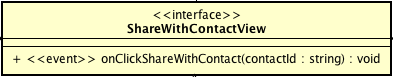
\includegraphics[scale=0.5]{Sezioni/SottosezioniST/img/app/ShareWithContactView.png}
	\caption{feature::sharewithcontact::ShareWithContactView}
\end{figure}

\begin{itemize}
\item \textbf{Descrizione}: Interfaccia che estende \texttt{GeneralView} che una volta implementata permette al presenter e allo sviluppatore di condividere la vista di una lista ad un utente.
\item \textbf{Utilizzo}: L'interfaccia viene utilizzata per disaccoppiare presenter e implementazione della vista, e visualizza i dati che gli vengono passati dal presenter.
\item \textbf{Attributi}: 
\item \textbf{Metodi}:
\item \textbf{Eventi}:
\begin{itemize}
\item \textit{public onClickShareWithContact(contactId:string):void}\\
	Evento che notifica tutti gli oggetti in ascolto che è stato cliccato il pulsante relativo alla condivisione con un utente.
	\\ \textbf{Parametri}: \begin{itemize}
	\item \textit{contactId:string}\\
	Id del contatto a cui condividere la lista.
	\end{itemize} 
\end{itemize}
\end{itemize}

\subsubsection{feature::sharewithcontact::view::ShareWithContactViewImpl}

\label{feature::sharewithcontact::view::ShareWithContactViewImpl}
\begin{figure}[ht]
	\centering
	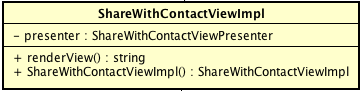
\includegraphics[scale=0.5]{Sezioni/SottosezioniST/img/app/ShareWithContactViewImpl.png}
	\caption{feature::sharewithcontact::view::ShareWithContactViewImpl}
\end{figure}

\begin{itemize}
\item \textbf{Descrizione}: Classe che implementa l'interfaccia \texttt{ShareWithContactView}, che permette al presenter e allo sviluppatore di condividere la vista di una lista con un utente.
\item \textbf{Utilizzo}: Classe utilizzata per condividere la view di una lista ad un utente.
\item \textbf{Attributi}: 
\begin{itemize}
\item \textit{private presenter:ShareWithContactViewPresenter}\\
	Il presenter associato alla view per condividere una lista ad un utente, al quale questa classe delega la gestione del comportamento della view stessa.
\end{itemize}
\item \textbf{Metodi}:
\begin{itemize}
\item \textit{public renderView():string}\\
	Genera il codice HTML CSS JS necessario per visualizzare la view.
\item \textit{public ShareWithContactViewImpl():ShareWithContactViewImpl}\\
	Il costruttore della classe ShareWithContactViewImpl.
\end{itemize}
\item \textbf{Eventi}:
\end{itemize}

\subsubsection{feature::sharewithcontact::presenter::ShareWithContactViewPresenter}

\label{feature::sharewithcontact::presenter::ShareWithContactViewPresenter}
\begin{figure}[ht]
	\centering
	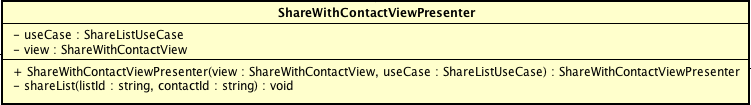
\includegraphics[scale=0.5]{Sezioni/SottosezioniST/img/app/ShareWithContactViewPresenter.png}
	\caption{feature::sharewithcontact::presenter::ShareWithContactViewPresenter}
\end{figure}

\begin{itemize}
\item \textbf{Descrizione}: Classe che rappresenta il presenter dedicato alla view per la condivisione di una lista ad un utente.
\item \textbf{Utilizzo}: Il presenter fa da tramite tra l'implementazione della view e la parte logica dell'applicazione, formattando i dati che verranno visualizzati nella view e manipolando gli input dell'utente per eseguire le operazioni predisposte.
\item \textbf{Attributi}: 
\begin{itemize}
\item \textit{private useCase:ShareListUseCase}\\
	Oggetto dedicato alla gestione della condivisione di una lista all'interno del database.
\item \textit{private view:ShareWithContactView}\\
	La view associata al presenter.
\end{itemize}
\item \textbf{Metodi}:
\begin{itemize}
\item \textit{private shareList(listId:string, contactId:string):void}\\
	Metodo che permette la condivisione di una lista ad un utente.
	\\ \textbf{Parametri}: \begin{itemize}
	\item \textit{listId:string}\\
	Id della lista da condividere.
	\item \textit{contactId:string}\\
	Id dell'utente a cui condividere la lista.
	\end{itemize} 
\item \textit{public ShareWithContactViewPresenter(useCase:ShareListUseCase, \\ view:ShareWithContactView):ShareWithContactViewPresenter}\\
	Il costruttore della classe ShareWithContactViewPresenter.
		\\ \textbf{Parametri}: \begin{itemize}
			\item \textit{useCase:ShareListUseCase}\\
			Oggetto dedicato alla gestione della condivisione di una lista all'interno del database.
			\item \textit{view:ShareWithContactView}\\
			La view necessaria alla costruzione del presenter.
\end{itemize} 
\item \textbf{Eventi}:
\end{itemize}
\end{itemize}

\subsubsection{usecase::ShareListUseCase}

\label{usecase::ShareListUseCase}
\begin{figure}[ht]
	\centering
	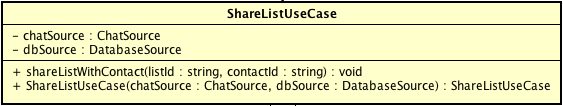
\includegraphics[scale=0.5]{Sezioni/SottosezioniST/img/app/ShareListUseCase.png}
	\caption{usecase::ShareListUseCase}
\end{figure}

\begin{itemize}
\item \textbf{Descrizione}: Classe dedicata alla gestione della condivisione di una lista all'interno del database.
\item \textbf{Utilizzo}: Classe utilizzata per la gestione della condivisione di una lista all'interno del database.
\item \textbf{Attributi}: 
\begin{itemize}
\item \textit{private chatSource:ChatSource}\\
	Riferimento di interfaccia a Rocket.chat.
\item \textit{private dbSource:DatabaseSource}\\
	Riferimento al database.
\end{itemize}
\item \textbf{Metodi}:
\begin{itemize}
\item \textit{public shareListWithContact(listId:string, contactId:string):void}\\
	Permettere di condividere la vista della lista ad un utente gestendo i relativi dati all'interno del database.
	\\ \textbf{Parametri}: \begin{itemize}
	\item \textit{listId:string}\\
	Id della lista da condividere.
	\item \textit{contactId:string}\\
	Id dell'utente a cui condividere la lista.
	\end{itemize} 
\item \textit{public ShareListUseCase(chatSource:ChatSource, dbSource:DatabaseSource):ShareListUseCase}\\
	Il costruttore della classe ShareListUseCase.
	\\ \textbf{Parametri}: \begin{itemize}
	\item \textit{chatSource:ChatSource}\\
	 	Riferimento di interfaccia a Rocket.chat.
	\item \textit{dbSource:DatabaseSource}\\
		Riferimento al database.
	\end{itemize} 
\end{itemize}
\item \textbf{Eventi}:
\end{itemize}

\subsubsection{feature::sharewithgroup::ShareWithGroupView}

\label{feature::sharewithgroup::ShareWithGroupView}
\begin{figure}[ht]
	\centering
	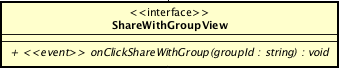
\includegraphics[scale=0.5]{Sezioni/SottosezioniST/img/app/ShareWithGroupView.png}
	\caption{feature::sharewithgroup::ShareWithGroupView}
\end{figure}

\begin{itemize}
\item \textbf{Descrizione}: Interfaccia che estende \texttt{GeneralView} che una volta implementata permette al presenter e allo sviluppatore di condividere la vista di una lista ad un gruppo di utenti.
\item \textbf{Utilizzo}: L'interfaccia viene utilizzata per disaccoppiare presenter e implementazione della vista, e visualizza i dati che gli vengono passati dal presenter.
\item \textbf{Attributi}: 
\item \textbf{Metodi}:
\item{Eventi}:
	\begin{itemize}
	\item \textit{public onClickShareWithGroup(groupId:string):void}\\
	Evento che notifica tutti gli oggetti in ascolto che è stato cliccato il pulsante relativo alla condivisione con un gruppo di utenti.										
	\\ \textbf{Parametri}: \begin{itemize}
			\item \textit{groupId:string}\\
			Id del gruppo a cui condividere la lista.
			\end{itemize} 
	\end{itemize}
\end{itemize}

\subsubsection{feature::sharewithgroup::view::ShareWithGroupViewImpl}

\label{feature::sharewithgroup::view::ShareWithGroupViewImpl}
\begin{figure}[ht]
	\centering
	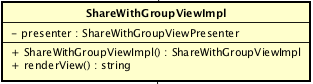
\includegraphics[scale=0.5]{Sezioni/SottosezioniST/img/app/ShareWithGroupViewImpl.png}
	\caption{feature::sharewithgroup::view::ShareWithGroupViewImpl}
\end{figure}

\begin{itemize}
\item \textbf{Descrizione}: Classe che implementa l'interfaccia \texttt{ShareWithGroupView}, che permette al presenter e allo sviluppatore di condividere la vista di una lista con un gruppo di utenti.
\item \textbf{Utilizzo}: Classe utilizzata per condividere la view di una lista ad un gruppo di utenti.
\item \textbf{Attributi}:
	\begin{itemize}
	\item \textit{private presenter:ShareWithGroupViewPresenter}\\
	Il presenter associato alla view per condividere una lista ad un gruppo di utenti, al quale questa classe delega la gestione del comportamento della view stessa.
	\end{itemize} 
\item \textbf{Metodi}:
	\begin{itemize}
	\item \textit{public ShareWithGroupViewImpl():ShareWithGroupViewImpl}\\
	Il costruttore della classe ShareWithGroupViewImpl.
	\item \textit{public renderView():string}\\
		Genera il codice HTML CSS JS necessario per visualizzare la view.
	\end{itemize}
\item{Eventi}:
\end{itemize}

\subsubsection{feature::sharewithgroup::presenter::ShareWithGroupViewPresenter}

\label{feature::sharewithgroup::presenter::ShareWithGroupViewPresenter}
\begin{figure}[ht]
	\centering
	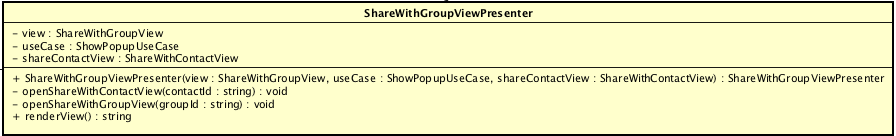
\includegraphics[scale=0.5]{Sezioni/SottosezioniST/img/app/ShareWithGroupViewPresenter.png}
	\caption{feature::sharewithgroup::presenter::ShareWithGroupViewPresenter}
\end{figure}

\begin{itemize}
\item \textbf{Descrizione}: Classe che rappresenta il presenter dedicato alla view per la condivisione di una lista ad un gruppo di utenti.
\item \textbf{Utilizzo}: Il presenter fa da tramite tra l'implementazione della view e la parte logica dell'applicazione, formattando i dati che verranno visualizzati nella view e manipolando gli input dell'utente per eseguire le operazioni predisposte.
\item \textbf{Attributi}: 
	\begin{itemize}
	\item \textit{private view:ShareWithGroupView}\\
			La view associata al presenter.
	\item \textit{private useCase:ShowPopupUseCase}\\
		Oggetto dedicato alla creazione del popup per la condivisione della lista.
	\item \textit{private shareContactView:ShareWithContactView}\\
		Oggetto che rappresenta la vista in cui selezionare gli utenti a cui condividere la lista.
	\end{itemize} 
\item \textbf{Metodi}:
	\begin{itemize}
	\item \textit{public ShareWithGroupViewPresenter(view:ShareWithGroupView, useCase:ShowPopupUseCase, \\ shareContactView:ShareWithContactView):ShareWithGroupViewPresenter}\\
	Il costruttore della classe ShareWithGroupViewPresenter.
			\\ \textbf{Parametri}: \begin{itemize}
			\item \textit{view:ShareWithGroupView}\\
			La view necessaria alla costruzione del presenter.
			\item \textit{useCase:ShowPopupUseCase}\\
			Oggetto dedicato alla creazione del popup per la condivisione della lista.
			\item \textit{shareContactView:ShareWithContactView}\\
					Oggetto che rappresenta la vista in cui selezionare gli utenti a cui condividere la lista.
			\end{itemize} 
	\item \textit{public renderView():string}\\
		Genera il codice HTML CSS JS necessario per visualizzare la view.
	\end{itemize}
\item{Eventi}:
\end{itemize}